\chapter*[Introdução]{Introdução}
\addcontentsline{toc}{chapter}{Introdução}

Este documento é definido como um conjunto de pesquisas e descri\c{c}\~oes de atividades que ir\~ao resultar em um projeto de melhorias que utilizam exclusivamente solu\c{c}\~oes tecnol\'ogicas para o Parque Urbano do Gama-DF. Esse projeto deve ser detalhado de modo a ser poss\'ivel uma futura utiliza\c{c}\~ao das ideias aqui descritas atrav\'es de simula\c{c}\~oes, esquem\'aticos e texto descritivo. 

\section{Contextualiza\c{c}\~ao}

O Parque Vivencial do Gama localiza-se na Regi\~ao Administrativa II do Gama, criada atrav\'es da Lei n.$^o$ 49/89 e do Decreto n.$^o$ 11.921/89 e formada por \'area urbana e rural. A \'area urbana \'e dividida em seis setores, sendo: Norte, Sul, Leste, Oeste, Central e de Ind\'ustria. O Parque Vivencial do Gama est\'a localizado no setor Norte (coordenadas 16 $^o$ 00`13.4``S 48 $^o$03`55.0``W), ocupando uma \'area de aproximadamente 52 mil m$^{2}$ \cite{COEX}. A Figura abaixo apresenta a imagem da \'area do parque.

\begin{figure}[H]
	\centering
	\label{Imagem do Parque Vivencial do Gama}
		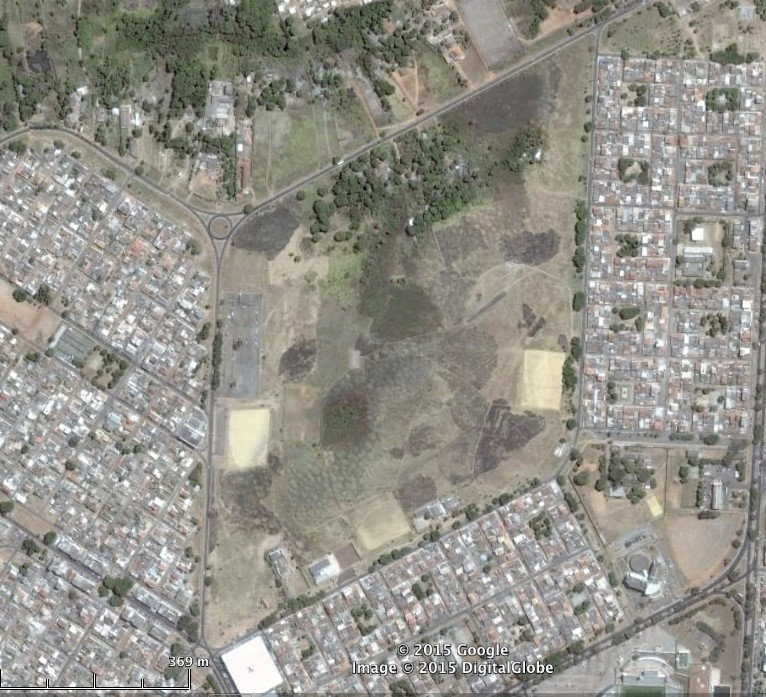
\includegraphics[keepaspectratio=true,scale=0.6]{introducao/ParqueVivencialGama.jpg}
	\caption{Imagem do Parque Vivencial do Gama}
	\small{Fonte: Google, 2015}
\end{figure}

A vegeta\c{c}\~ao que existente no Parque est\'a ligada ao Bioma Cerrado, mas no momento n\~ao se encontra preservado restando apenas esp\'ecies do tipo buritis, pata-de-vaca (Bauhinia variegata) e vegeta\c{c}\~ao rasteira.  O solo do parque \'e hidrom\'orfico, ou seja, tem excesso de umidade. Nessa \'area tamb\'em h\'a nascentes o que limita a constru\c{c}\~ao civil no pr\'oprio parque perante a Lei N$^{o}$ 12.651/12 - C\'odigo Florestal, a qual prev\^e prote\c{c}\~ao \`a \'area de nascentes. Abaixo, tem-se as figuras abaixo apresentam respectivamente, a vegeta\c{c}\~ao e as nascentes \cite{COEX}.

\begin{figure}[H]
	\centering
	\label{Imagem do Parque Vivencial do Gama}
		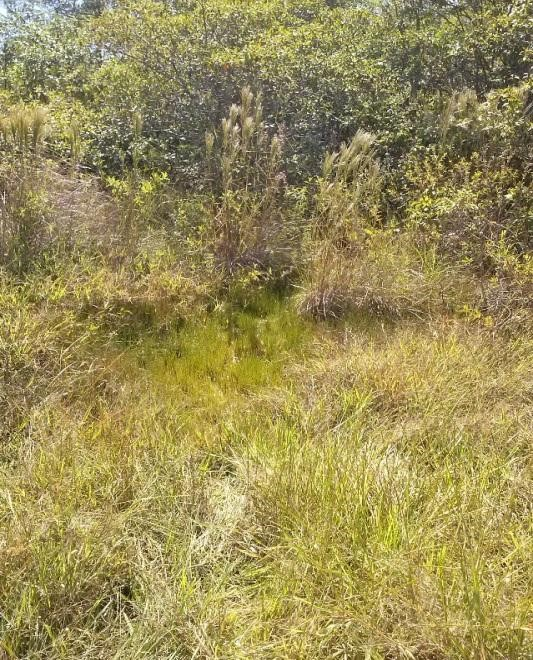
\includegraphics[keepaspectratio=true,scale=0.4]{introducao/VegatacaoTipica.jpg}
	\caption{Imagem da vegata\c{c}\~ao T\'ipica.}
	\small{Fonte: Administra\c{c}\~ao do Gama, 2015}
\end{figure}

\begin{figure}[H]
	\centering
	\label{Imagem do Parque Vivencial do Gama}
		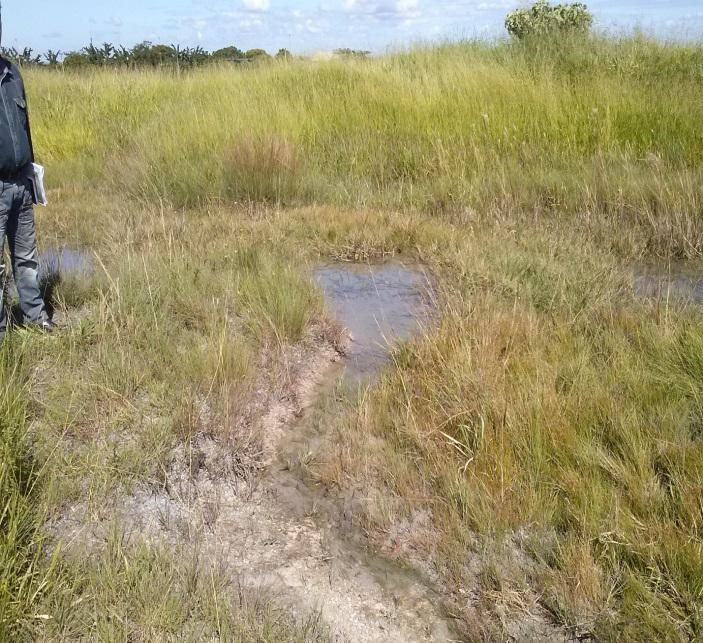
\includegraphics[keepaspectratio=true,scale=0.4]{introducao/Nascentes.jpg}
	\caption{Imagem de uma das nascentes.}
	\small{Fonte: Administra\c{c}\~ao do Gama, 2015}
\end{figure}

Inicialmente o Parque Vivencial do Gama foi projetado com uma infraestrutura que possu\'ia \textit{playground}, quadras poliesportivas, pistas de \textit{cooper} e ciclovia, espa\c{c}os de conviv\^encia, entre outros aparatos \cite{Ibram}. Al\'em disso, possui tamb\'em banheiros, quiosques, quatro campos de futebol e o pr\'edio da administra\c{c}\~ao. Mas, segundo integrantes do grupo que visitaram o parque, todos esses itens est\~ao em p\'essimas condi\c{c}\~oes de conservamento e de uso ou est\~ao sendo usados para outros fins, como por exemplo, o \textit{playground} que \'e usado por usu\'arios de drogas como um local de conviv\^encia. 